% !TEX root = main.tex
%%%% Colour Palette %%%%%
\definecolor{black1}{RGB}{0,0,0}
\definecolor{orange1}{RGB}{230,159,0}
\definecolor{skyblue}{RGB}{86,180,233}
\definecolor{blueishgreen}{RGB}{0,158,115}
\definecolor{yellow}{RGB}{240,228,66}
\definecolor{blue1}{RGB}{0,114,178}
\definecolor{vermillion}{RGB}{213,94,0}
\definecolor{reddishpurple}{RGB}{204,121,167}
%%%%%% Block Styles %%%%%%%%%%%%%%%%%%%%%%%%%%%%
\tikzstyle{decision} = [diamond, draw, fill=blueishgreen,
    text width=4.5em, text badly centered, node distance=3cm, inner sep=0pt]
\tikzstyle{block} = [rectangle, draw, fill=skyblue,
    text width=5em, text centered, rounded corners, minimum height=4em]
\tikzstyle{line} = [draw, -latex']
\tikzstyle{cloud} = [draw, ellipse,fill=yellow, text width=5.5em, node distance=3.5cm,
    minimum height=2em]
%%%%%%%%%%%%%%%%%%%%%%%%%%%%%%%%%%%%%%%%%%%%%



\chapter{Simulation}\label{cha:simulations}

  Using the previous theory, simulating the rocket's ignition phase can be done using only a fairly small sample of data. Molar masses, gas constants and the like are all table constants. Given ambient pressure $P_0$, temperature $T_0$ and chamber volume $V_\text{chamber}$, initial conditions can be calculated. As the rocket takes off, using the mass flow $\dot{m}$ and fraction of oxygen being consumed in combustion $f$, we can compute the rocket's performance at all times assuming isentropic flow. The inner pressure and temperature can be found by calculating the flow into and out of the rocket, as well as the energy released in the various chemical reactions.
%
\begin{figure}
	\centering
	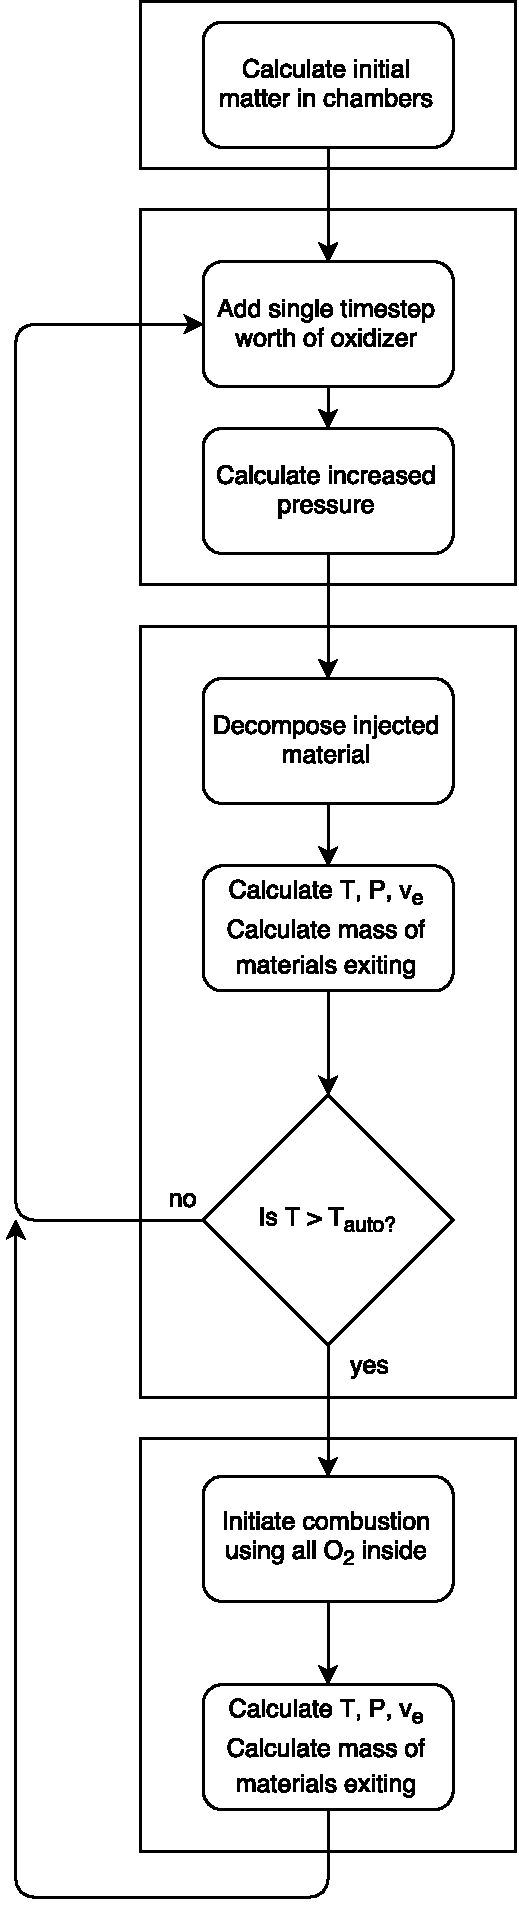
\includegraphics[width=0.45\textwidth]{rocketflowchart.pdf}
	\caption{Scheme showing the implementation of the rocket's ignition algorithm.}
	\label{fig:flowchart}
\end{figure}


\section{Implementation}

  The rocket engine's ignition algorithm is based on the previous assumptions. Figure \ref{fig:flowchart} shows a flowchart of the ignition algorithm. The implemented algorithm is divided into four parts, which determine the rocket's performance at various stages. The first stage is the rocket's pre-launch conditions, eg. amount of substance $n$, pressure $P$ and temperature $T$. The second stage is injection of oxidizer into the pre--combustion (or decomposition) chamber. The amount of injected oxidizer is equivalent to the injection nozzle's flow per time step $\Delta t$ in every iteration. This is followed by recalculating the rocket's conditions. After the initial matter has been injected, decomposition starts. This is the third stage of the algorithm. Post decomposition, the temperature, pressure, exit velocity $v_e$ and exit mass can be found. The temperature is compared to the autoignition temperature $T_\text{auto}$: If higher, combustion of material still contained inside the rocket starts. Otherwise, more oxidizer is injected and decomposed until the energy released during decomposition heats the interior to autoignition temperatures. The final stage occurs when temperatures are large enough to allow combustion. Combustion expends \emph{all} the available oxygen inside the rocket during every iteration. This means, that if $T_\text{auto} \approx T_\text{amb}$, combustion occurs instantaneously, using only the oxygen released by the first time step's oxidizer. If, however, $T_\text{auto} > T_\text{amb}$ (as it is in our case), combustion occurs a certain time later, allowing oxygen to accumulate inside the chamber.

\section{Results}

  \begin{figure}
  	\centering
  	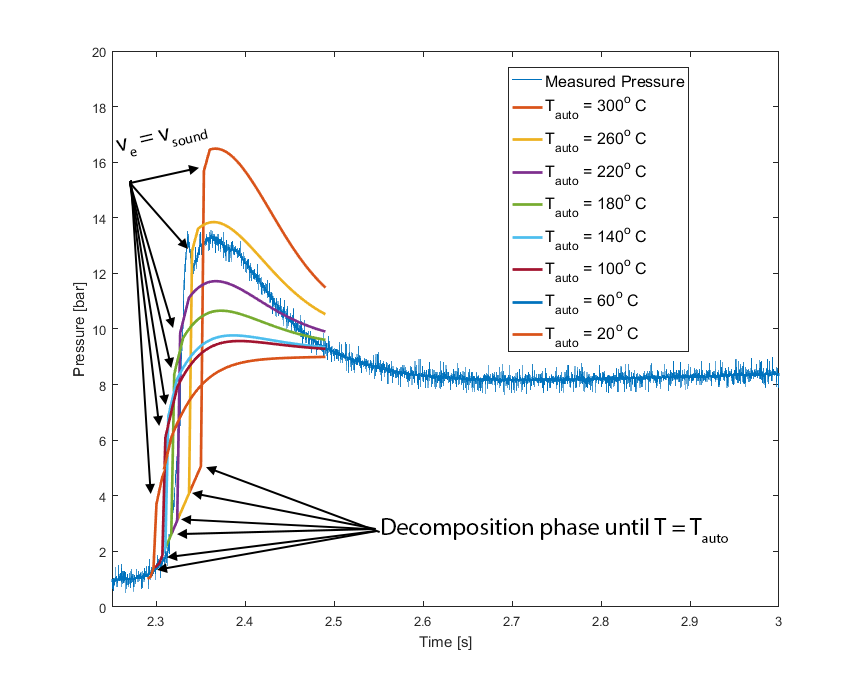
\includegraphics[width=\textwidth]{pressureovertime3}
  	\caption{Pressure over time for different autoignition temperatures $T_\text{auto}$. The highest peak is given by the highest autoignition temperature. The first linear phase at the bottom is where decomposition happens without combustion. When the curve breaks, combustion occurs. Instantaneously after combustion, all models' exit velocities reach the speed of sound.}
  	\label{fig:pressureovertime}
  \end{figure}

  The simulation shows promising results in the description of the hybrid engine's pressure spikes. As it appears from figure \ref{fig:pressureovertime}, the higher the autoignition temperature the higher the peak pressure is. Thereto, the higher the peak, the later combustion takes place. This is to be expected, as a higher autoignition point allows more oxygen to accumulate in the chamber which of course takes more time. All of the simulations tend toward a steady-state at the end, where they would eventually meet at the design--pressure. The yellow, low auto-ignition point of $\SI{60}{\celsius}$ steadily and cleanly tend toward the design--pressure, as would be preferred for the hybrid rocket. The steady increase ensures no rapid combustion happens, and transitions between the ignition states flow without problem. This result proposes the hypothesis, that a reduction of the autoignition temperature, or the presence of a pilot flame might be able to extinguish the unwanted spiking behavior.

  \begin{figure}
  	\centering
  	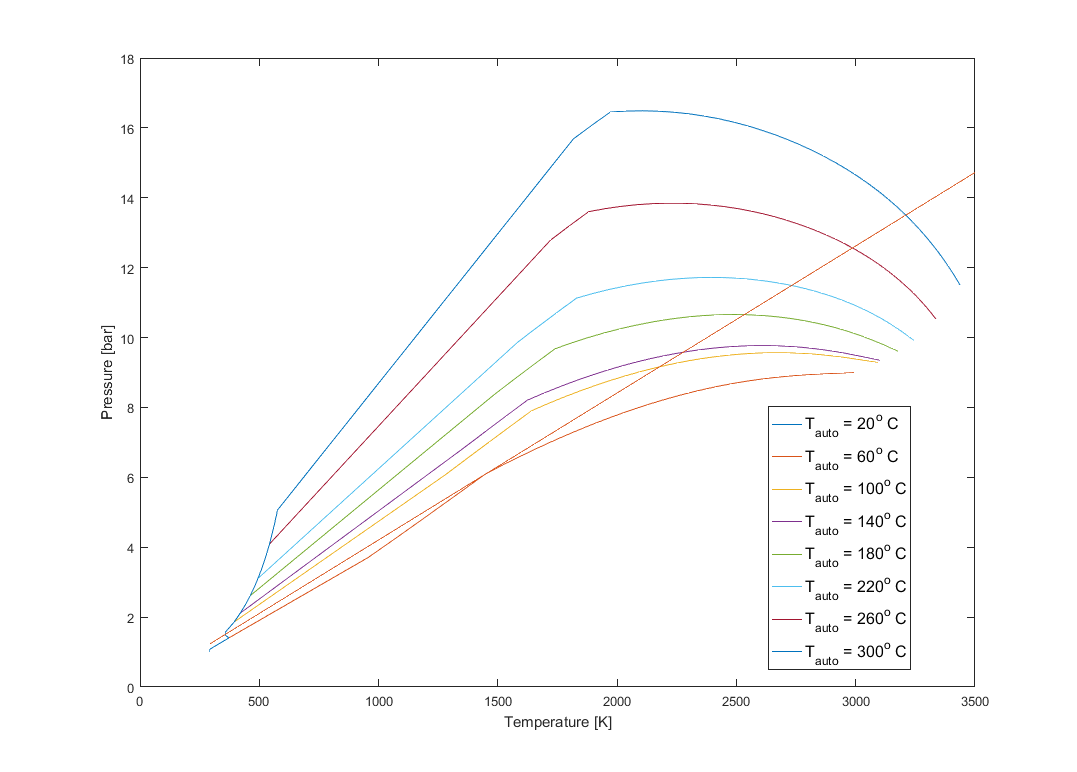
\includegraphics[width=\textwidth]{pressurepertemperature}
  	\caption{Pressure per temperature for different autoignition temperatures $T_\text{auto}$. The straight line is a theoretical fit assuming constant amount of substance $n$.}
  	\label{fig:pressurepertemperature}
  \end{figure}

  In figure \ref{fig:pressurepertemperature} we see the pressure plotted against temperature in the simulation, with a theoretical fit of the rocket's design values. After initial spiking, the pressure drops as the temperature increases up to very large values of almost $\SI{3500}{\kelvin}$. The pressure should stabilize steadily towards the end, but all simulations show a trend of pressure dropping with increasing pressure. However, the rocket is designed to work at a temperature of $\SI{2500}{\kelvin}$, and the pressure values around this area varies between $\SI{8.8}{\bar}$ and $\SI{16.2}{\bar}$ -- somewhat within the design pressure of $\SI{10}{\bar}$.

  %
  % \section{Stage one: Injection}
  %
  %
  %
  % \section{Stage two: Decomposition}
  % \section{Stage three: Combustion}
  % \section{Stage four: Thrust}
  %
  %
  % \begin{tikzpicture}[node distance = 3cm, auto]
  %     % Place nodes
  %     \node [block] (const) {Define constants};
  %       \node [cloud, left of=const] (constvars) {$T_{amb}$, chamber dim., etc.};
  %     \node [block, below of=const] (inj) {Define injection rates per second};
  %       \node [cloud, left of=inj] (injvars) {$\dot{n}_{H_2O_2,1}$ $\dot{n}_{H_2O,1}$};
  %     \node [block, below of=inj] (dec) {Define decomposition rates per second};
  %       \node [cloud, left of=dec] (decvars) {$\dot{n}_{H_2O_2,2}$ $\dot{n}_{H_2O,2}$ $\dot{n}_{O_2,2}$};
  %     \node [block, below of=dec] (com) {Define combustion rates per second};
  %       \node [cloud, left of=com] (comvars) {$\dot{n}_{H_2O,3}$ $\dot{n}_{O_2,3}$ $\dot{n}_{CO_2,3}$};
  %     \node [block, below of=com] (exha) {Define exhaustion mass flow};
  %       \node [cloud, left of=exha] (exhavars) {$\dot{m}_{pla,3}$};
  % %%%% Defining more relavant stuff %%%%%
  %     \node [block, below of=exha] (mflow) {Define mass flow rates $n$ per time step $dt$ to find enthalpy};
  %       \node [cloud, left of=mflow] (mflowvars) {$m_{tot,n} = \sum\limits_{\text{chem.} 1}^{\text{chem. k}} \dot{n}_j \cdot dt$};
  %     \node [block, right of=mflow] (mfrac) {Calculate mass fraction in flow rates to calculate enthalpy leaving rocket later};
  %     \node [block, above of=mfrac, node distance=6cm] (refent) {Calculate reference enthalpy in decomposition and combustion states};
  %       \node [cloud, right of=refent] (refentvars) {$H = \sum \dot{m}_{j} \cdot H_j(P,T) + \Delta h_{dec,com} \cdot \dot{m}_\chem{H_2O_2} \cdot dt$};
  %     \node [decision, right of=const, node distance=5cm] (next) {Passes static data into $P$ and $T$ calculations};
  %
  %
  %     % Draw edges
  %     \path [line] (const) -- (inj);
  %     \path [draw] (const) -- (constvars);
  %     \path [line] (inj) -- (dec);
  %     \path [draw] (inj) -- (injvars);
  %     \path [line] (dec) -- (com);
  %     \path [draw] (dec) -- (decvars);
  %     \path [line] (com) -- (exha);
  %     \path [draw] (com) -- (comvars);
  %     \path [draw] (exha) -- (exhavars);
  %     \path [line] (exha) -- (mflow);
  %     \path [draw] (mflow) -- (mflowvars);
  %     \path [line] (mflow) -- (mfrac);
  %     \path [line] (mfrac) -- (refent);
  %     \path [draw] (refent) -- (refentvars);
  %     \path [line] (refent) -- (next);
  % \end{tikzpicture}
  %
  % INSERT FLOWCHART OF SECONDARY PART WHEN POWERPOINT WORKS



% \begin{tikzpicture}[node distance = 2cm, auto]
%     % Place nodes
%     \node [block] (init) {initialize model};
%     \node [cloud, left of=init] (expert) {expert};
%     \node [cloud, right of=init] (system) {system};
%     \node [block, below of=init] (identify) {identify candidate models};
%     \node [block, below of=identify] (evaluate) {evaluate candidate models};
%     \node [block, left of=evaluate, node distance=3cm] (update) {update model};
%     \node [decision, below of=evaluate] (decide) {is best candidate better?};
%     \node [block, below of=decide, node distance=3cm] (stop) {stop};
%     % Draw edges
%     \path [line] (init) -- (identify);
%     \path [line] (identify) -- (evaluate);
%     \path [line] (evaluate) -- (decide);
%     \path [line] (decide) -| node [near start] {yes} (update);
%     \path [line] (update) |- (identify);
%     \path [line] (decide) -- node {no}(stop);
%     \path [line,dashed] (expert) -- (init);
%     \path [line,dashed] (system) -- (init);
%     \path [line,dashed] (system) |- (evaluate);
% \end{tikzpicture}
